
\documentclass[12pt]{amsart}
\usepackage{geometry} % see geometry.pdf on how to lay out the page. There's lots.
\geometry{a4paper} % or letter or a5paper or ... etc
% \geometry{landscape} % rotated page geometry
\usepackage{graphicx} %插入图片的宏包
\usepackage{float} %设置图片浮动位置的宏包
\usepackage{subfigure} %插入多图时用子图显示的宏包
% See the ``Article customise'' template for come common customisations

\title{}
\author{}
\date{} % delete this line to display the current date

%%% BEGIN DOCUMENT
\begin{document}

\section{Preliminary Design}

\begin{figure}[H] %H为当前位置,!htb为忽略美学标准,htbp为浮动图形
\centering %图片居中
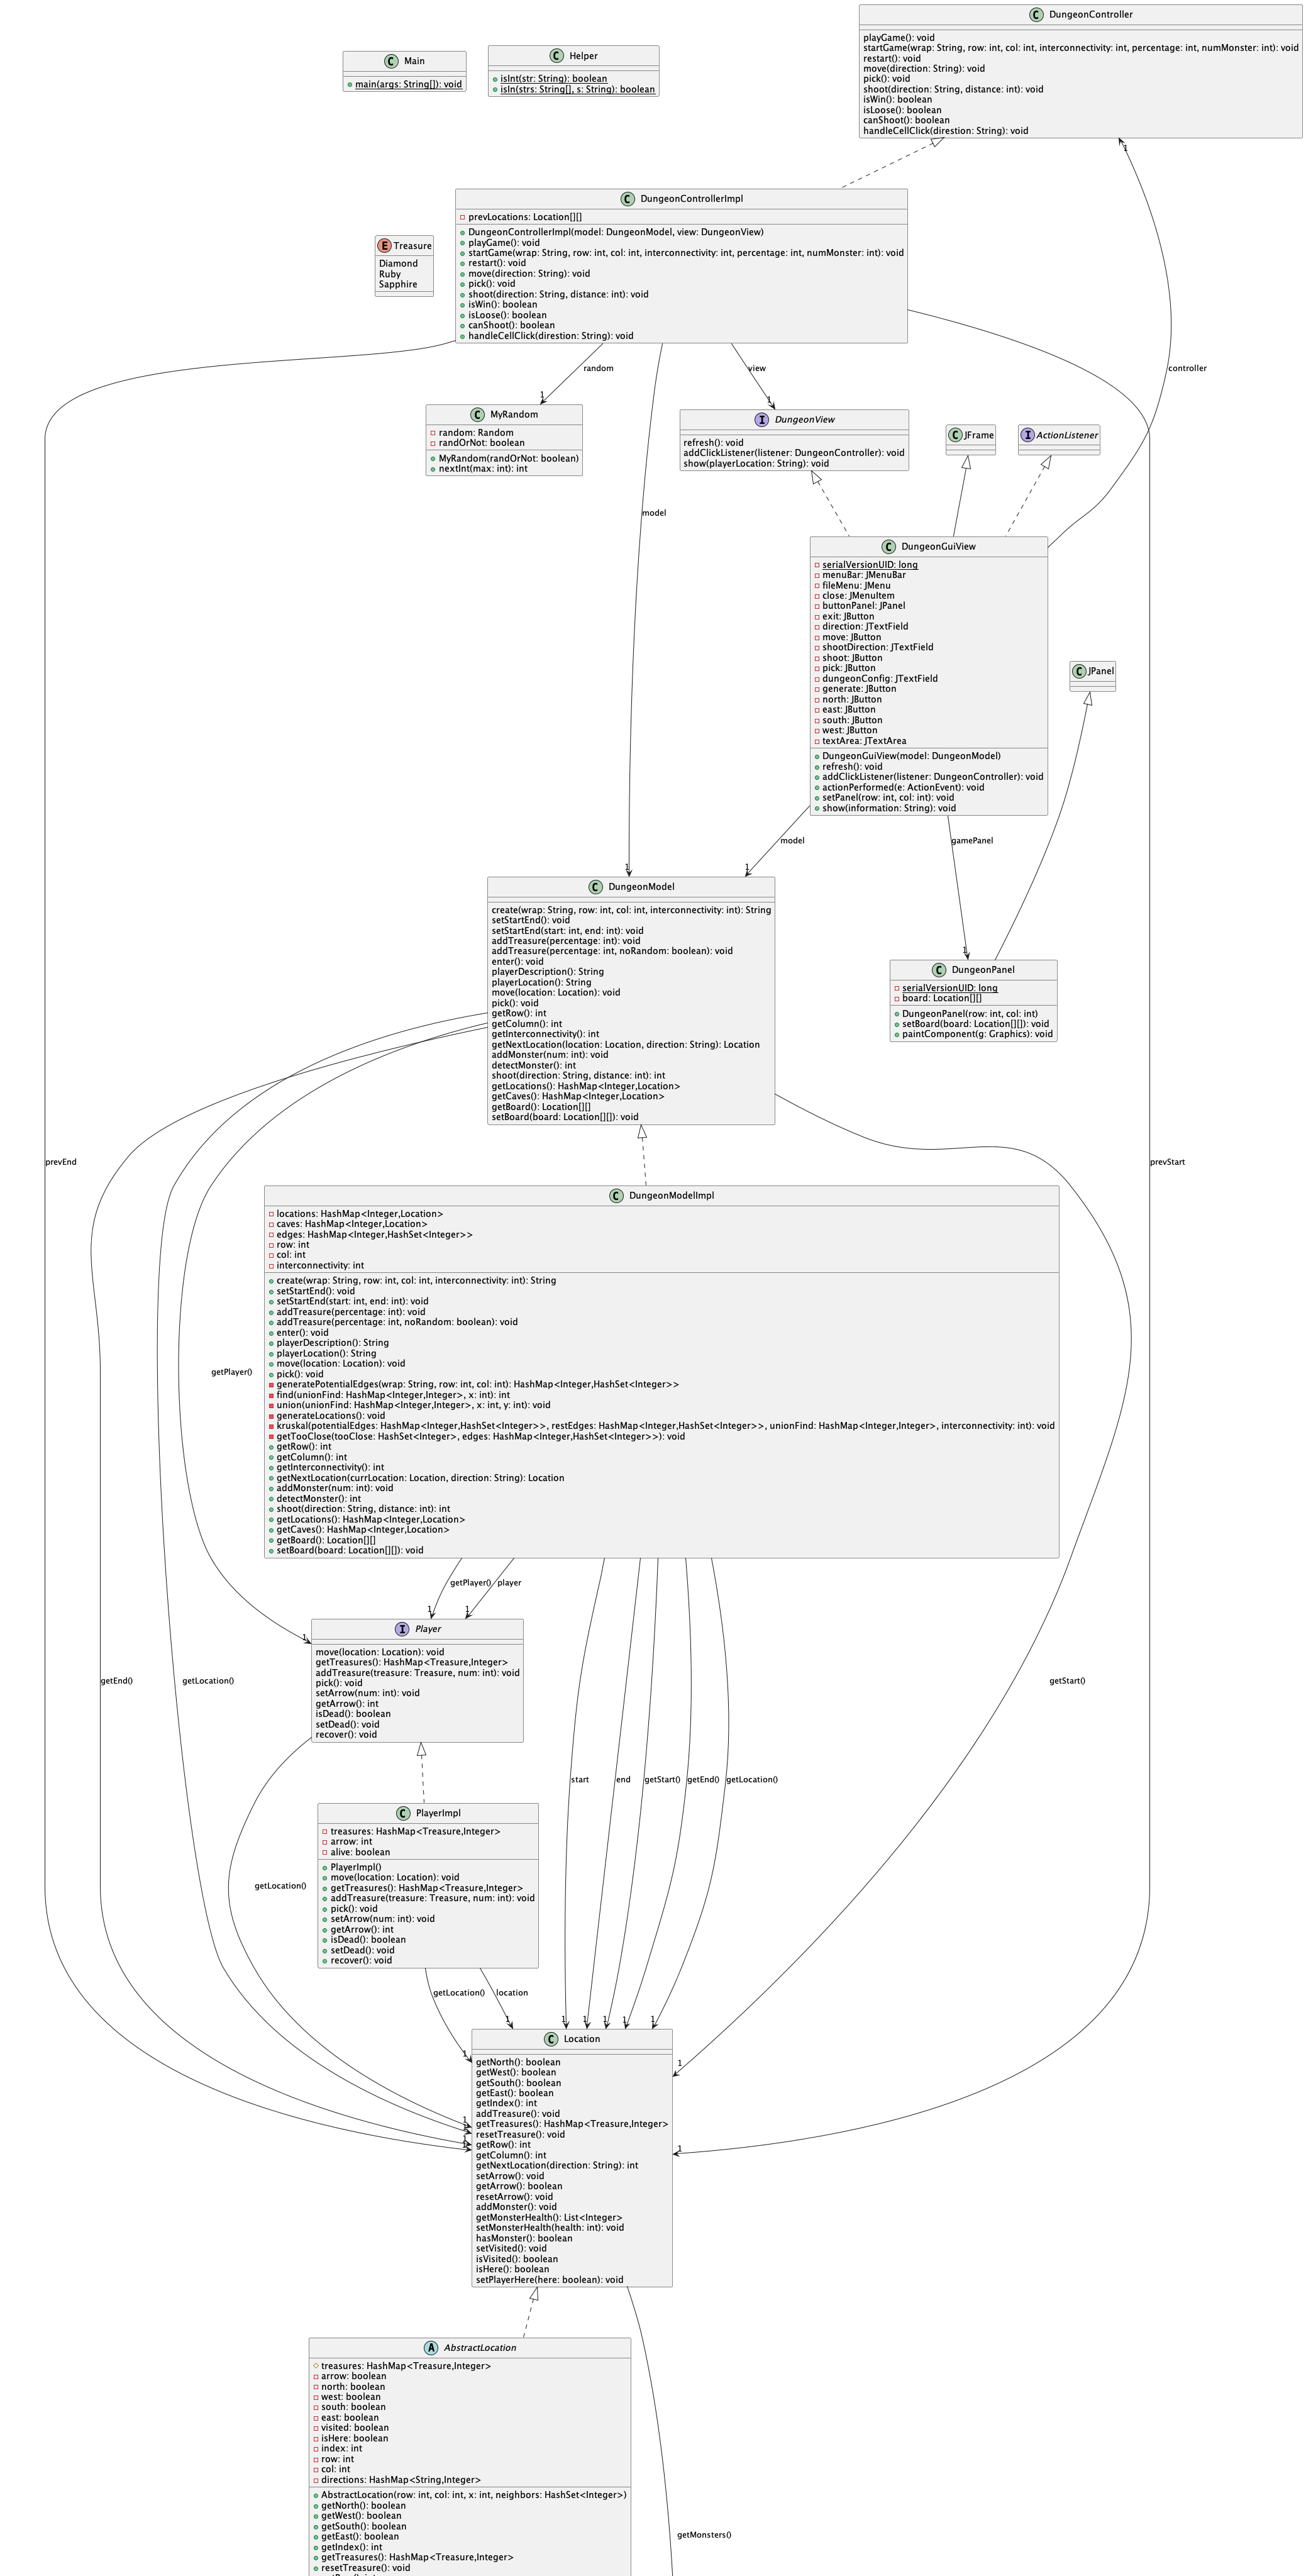
\includegraphics[width=1\textwidth]{uml.png} %插入图片,[]中设置图片大小,{}中是图片文件名
\end{figure}

\newpage

\begin{table}[htbp]
   %\topcaption{Table captions are better up top} % requires the topcapt package
   \begin{tabular}{@{} lll @{}} % Column formatting, @{} suppresses leading/trailing space

      Method     & Input & Expected \\
         addArrow   & Percentage of location with arrow    &  Correct percentage \\
         shoot & Specify direction and distance & Hurt monster if there exists\\
         move & String of direction & Controller moves model successfully\\
         printInformation & Nothing & Controller successfully print information associated with current location\\
         pick & Nothing & Controller control model to pick arrow and treasure\\
    
    \end{tabular}
\end{table}

\newpage

\section{Final Design}

\begin{figure}[H] %H为当前位置,!htb为忽略美学标准,htbp为浮动图形
\centering %图片居中
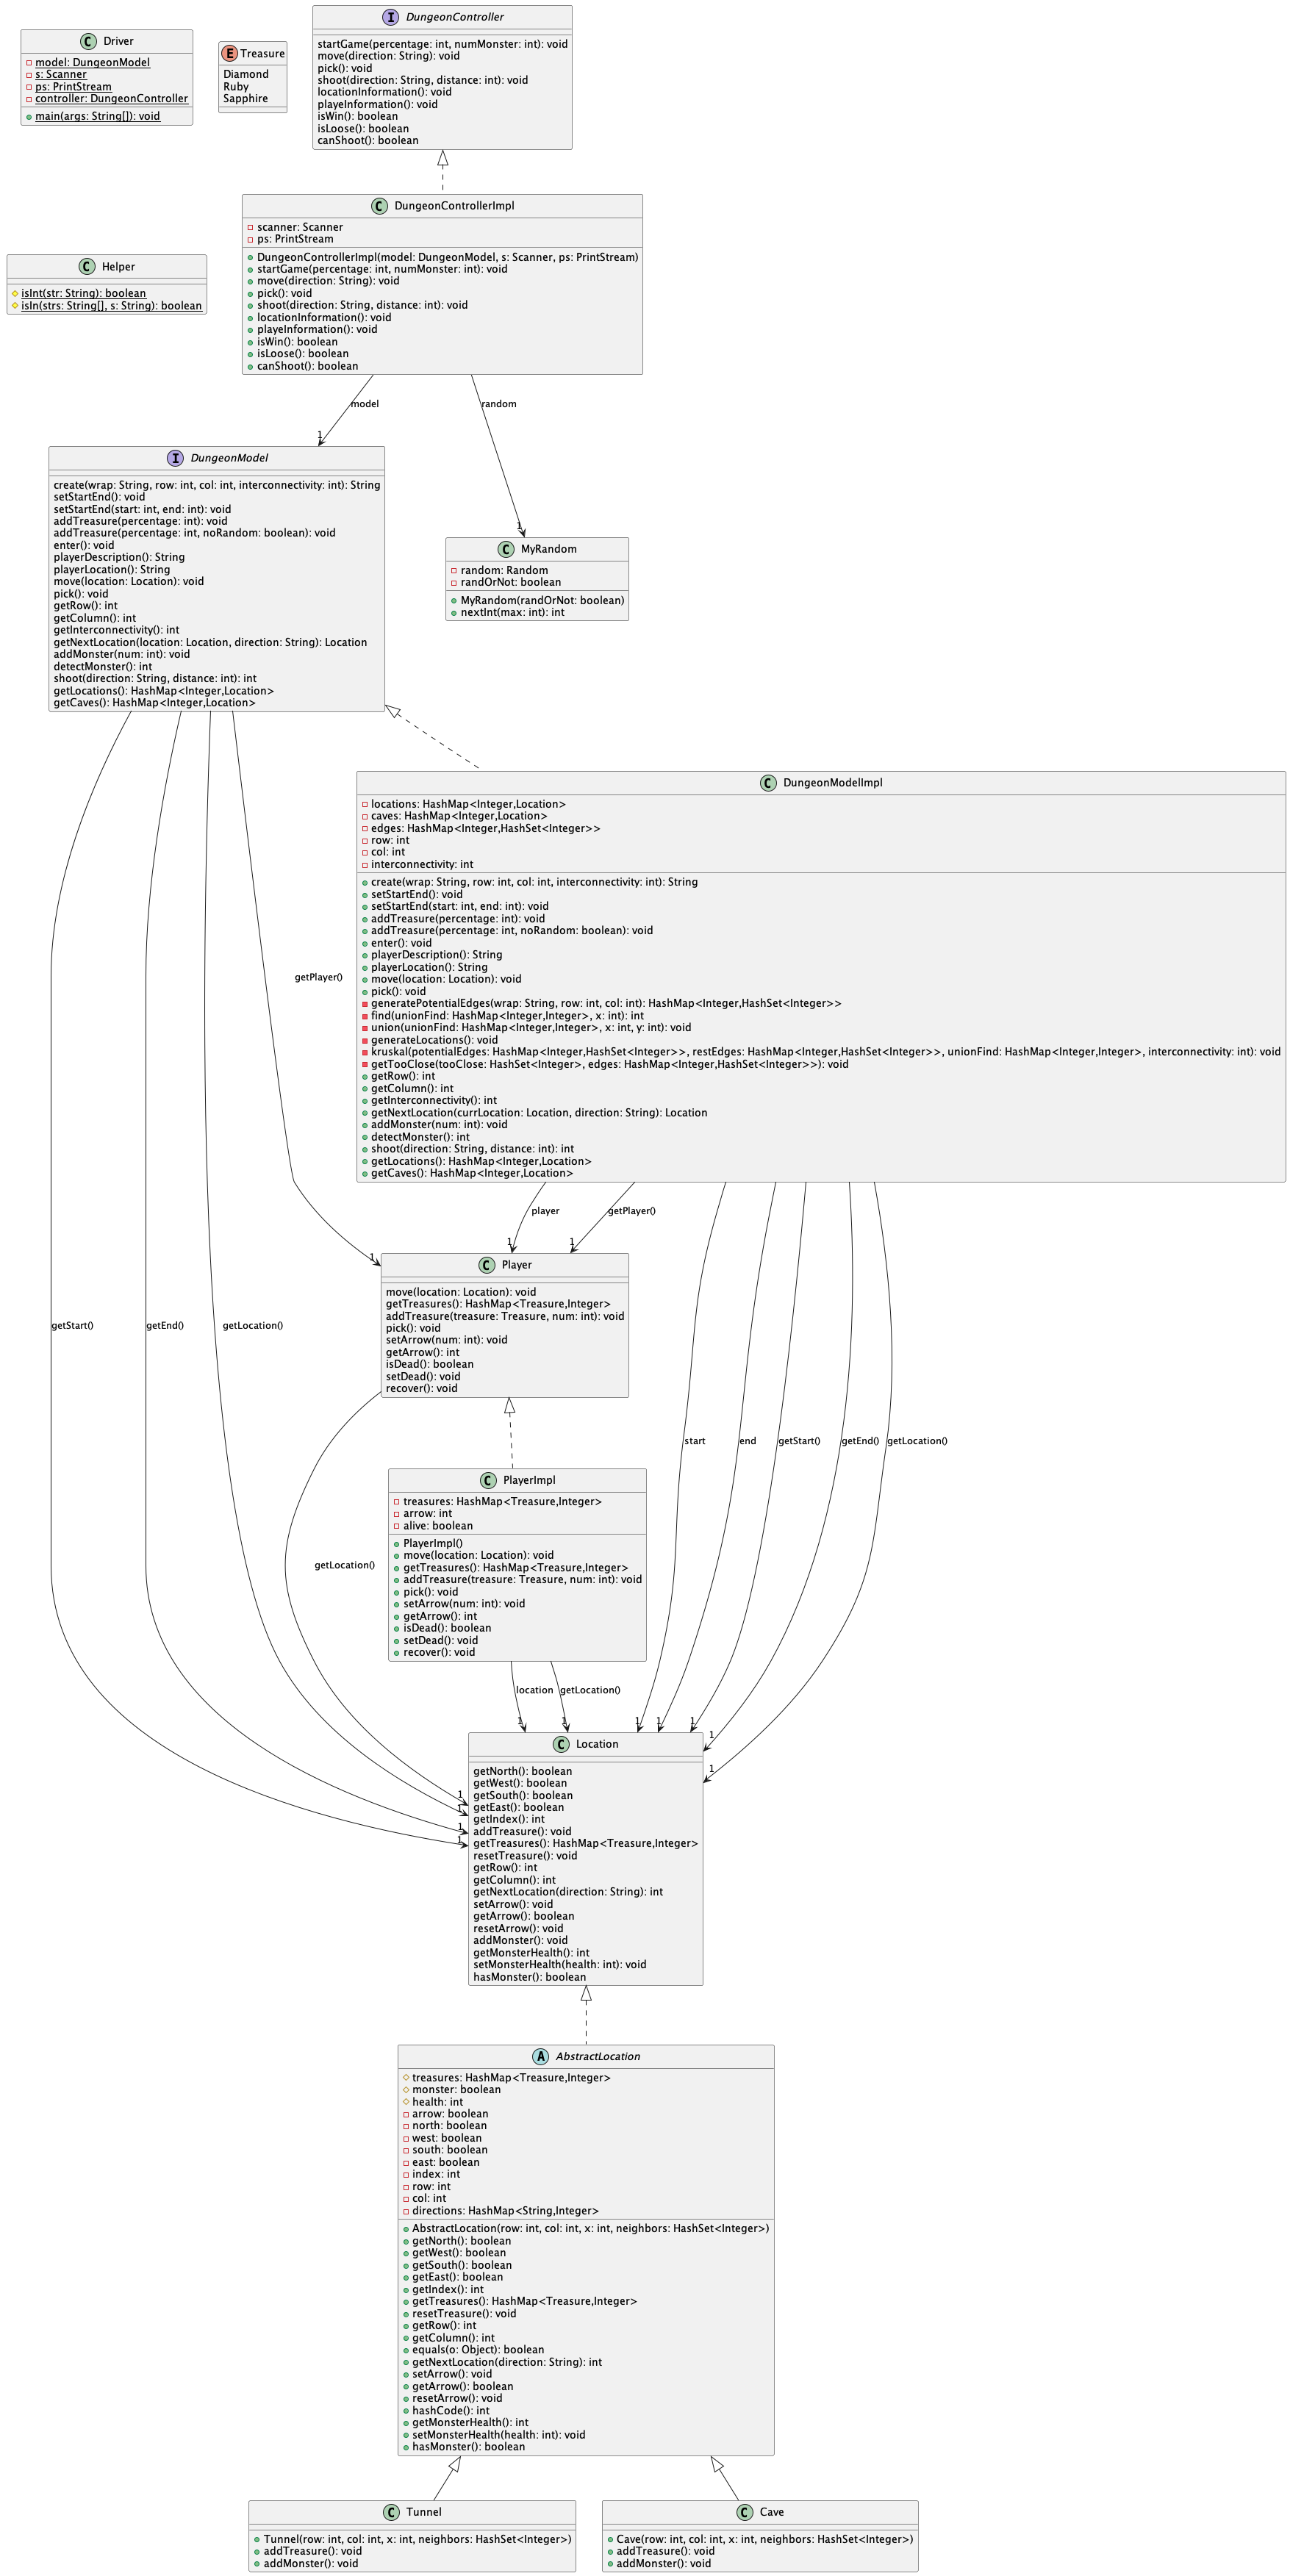
\includegraphics[width=1\textwidth]{final_uml.png} %插入图片,[]中设置图片大小,{}中是图片文件名
\end{figure}

\newpage

\begin{table}[htbp]
   %\topcaption{Table captions are better up top} % requires the topcapt package
   \begin{tabular}{@{} lll @{}} % Column formatting, @{} suppresses leading/trailing space

      Method     & Input & Expected \\
         monster at end   & NA    &  monster is at end \\
         monster added & 1 &  1 monster is added to model\\
         smell of 1 monster & NA & less smell of a monster\\
         smell of 2 monster & NA & strong smell of 2 monster\\
         add arrow & 1 & 1 arrow is added\\
         pick arrow & NA & player can pick up arrow\\
         shoot arrow & direction, distance & player shoot  at specified direction and distance\\
         arrow travel through locations & direction, distance & successful travel\\
         arrow miss monster & direction, distance & correct direction with wrong distance, arrow miss monster\\
         player killed & enter a location with monster & player dead\\
         can survive if monster is injured & repeat 100 times  & may survive\\
         kill monster & shoot twice & monster killed\\
         controller move & direction & move to specified direction\\
         controller pick & pick & successfully pick\\
         controller shoot & direction, distance & controller shoot success\\
         
    \end{tabular}
\end{table}



\end{document}



